% 
%  chapter3.tex
%  ISELthesis
%  
%  Created by Matilde Pós-de-Mina Pato on 2012/10/09.
%
\chapter{Metodologia e Arquitetura da Solução}
\label{cha:metodologia-arquitetura}
Neste capítulo é apresentada a metodologia adotada para a construção e avaliação de um sistema de recomendação baseado em Grafos de Conhecimento para descoberta biomédica de fármacos. A solução proposta parte de dados biomédicos previamente extraídos e estruturados através da ferramenta \emph{MedJsonify}~\cite{pereira2025mapping}, utilizada neste trabalho como uma infraestrutura externa de pré-processamento e não como uma contribuição desenvolvida no âmbito desta dissertação. Com base nestes dados, é construído um Grafo de Conhecimento biomédico multi-relacional, no qual fármacos, doenças, ingredientes e genes constituem as entidades, e as respetivas relações são representadas por tripletos canónicos.

A arquitetura da solução foi organizada de forma modular, separando a etapa de construção do grafo da etapa do desenvolvimento dos modelos de aprendizagem. Numa primeira fase, o módulo de construção do grafo transforma os dados estruturados em tripletos no formato \emph{src, rel, dst}, aplica processos de normalização e resolução de entidades, e produz diferentes versões do grafo que servirá de base para a futura aplicação dos modelos de aprendizagem escolhidos. Numa segunda fase, estes tripletos são convertidos em artefactos adequados ao treino desses modelos, sendo a tarefa principal formulada como \emph{disease-to-drug recommendation}: dada uma patologia, o sistema deve ordenar os fármacos candidatos pela probabilidade de apresentarem uma associação terapêutica relevante.

O modelo principal avaliado é uma \acrshort{rgcn}~\cite{schlichtkrull2018modeling}, adaptada ao contexto desta dissertação para aprendizagem em grafos biomédicos multi-relacionais, sendo comparada com uma abordagem \emph{content-based} desenvolvida como \emph{baseline}. A avaliação experimental recorre a métricas de ranking, nomeadamente \emph{Mean Reciprocal Rank} e \emph{Hits@k}, permitindo analisar a capacidade dos modelos em posicionar associações terapêuticas verdadeiras entre os primeiros resultados recomendados.

\section{Fontes de Dados e Caracterização do Dataset}
\label{sec:aquisicao-caracterizacao}
A construção de um \acrshort{kg} coerente e relevante do ponto de vista biomédico é determinante para a qualidade das previsões produzidas pelos modelos de aprendizagem relacional. Nesta secção, descrevem-se as fontes de dados que servem de base ao trabalho, o papel da ferramenta \emph{MedJsonify} no pré-processamento inicial e a forma como os dados estruturados resultantes são posteriormente utilizados para construir um dataset preparado para a tarefa de recomendação.

\subsection{Fontes de Dados e Pré-processamento Externo}
As fontes de dados utilizadas dividem-se em dois grupos complementares. O primeiro corresponde a fontes regulatórias e farmacêuticas, utilizadas para obter informação sobre medicamentos, ingredientes, formulações, vias de administração e outras informações dos respetivos rótulos oficiais. Este grupo inclui o \emph{DailyMed}~\cite{dailymed}, o \emph{Orange Book}~\cite{orangebook} e o \emph{Purple Book}~\cite{purplebook}, cujos dados são previamente processados pela ferramenta externa \emph{MedJsonify}~\cite{pereira2025mapping}.

O dataset utilizado corresponde a uma extração realizada num período específico das fontes regulatórias. Em particular, os dados provenientes do \emph{DailyMed} incluem ficheiros XML dos meses de julho, agosto e novembro de 2025, enquanto os dados do \emph{Orange Book} e do \emph{Purple Book} correspondem às versões de novembro de 2025. A seleção deste período de extração teve como objetivo utilizar a informação mais recente disponível à data da recolha, mantendo simultaneamente um volume de dados compatível com os recursos computacionais disponíveis. Esta delimitação é importante para a reprodutibilidade do trabalho, uma vez que as fontes regulatórias são atualizadas periodicamente e diferentes datas de extração podem originar variações no conjunto de medicamentos, ingredientes e informação textual disponível.

Importa salientar que o \emph{MedJsonify} não foi desenvolvido no âmbito desta dissertação. Neste trabalho, esta ferramenta é utilizada exclusivamente como uma infraestrutura de pré-processamento, responsável pela conversão de ficheiros heterogéneos em objetos JSON estruturados e pela aplicação de métodos de reconhecimento de entidades biomédicas. A contribuição desta dissertação inicia-se na importação desses JSONs, envolvendo a normalização e resolução de entidades, a construção dos tripletos canónicos, o enriquecimento do grafo de conhecimento e a preparação dos dados para o desenvolvimento, treino e avaliação dos modelos de recomendação.

O segundo grupo corresponde a fontes biomédicas orientadas para conhecimento molecular, utilizadas para enriquecer o grafo de conhecimento com relações entre doenças, genes e fármacos. Em particular, o \emph{Open Targets} fornece associações entre patologias e genes, representadas através da relação \texttt{ASSOCIATED\_WITH\_GENE}. Adicionalmente, o \emph{DGIdb} disponibiliza informação sobre interações entre fármacos e genes, permitindo incorporar a relação \texttt{INTERACTS\_WITH\_GENE}. A integração destas fontes complementa a informação clínica originalmente disponível, introduzindo conhecimento que estabelece ligações entre doenças, genes e fármacos no grafo de conhecimento.

\paragraph{DailyMed}
O \emph{DailyMed} constitui a fonte oficial para a consulta de rótulos de medicamentos aprovados pela FDA. Estes rótulos seguem o padrão \emph{Structured Product Labeling} (SPL), um formato XML que organiza informação regulatória e clínica de forma hierárquica e normalizada. No conjunto de dados de entrada, esta fonte fornece informação textual relevante para a identificação de medicamentos, ingredientes, indicações terapêuticas e contraindicações.

\begin{figure}[H]
    \centering
    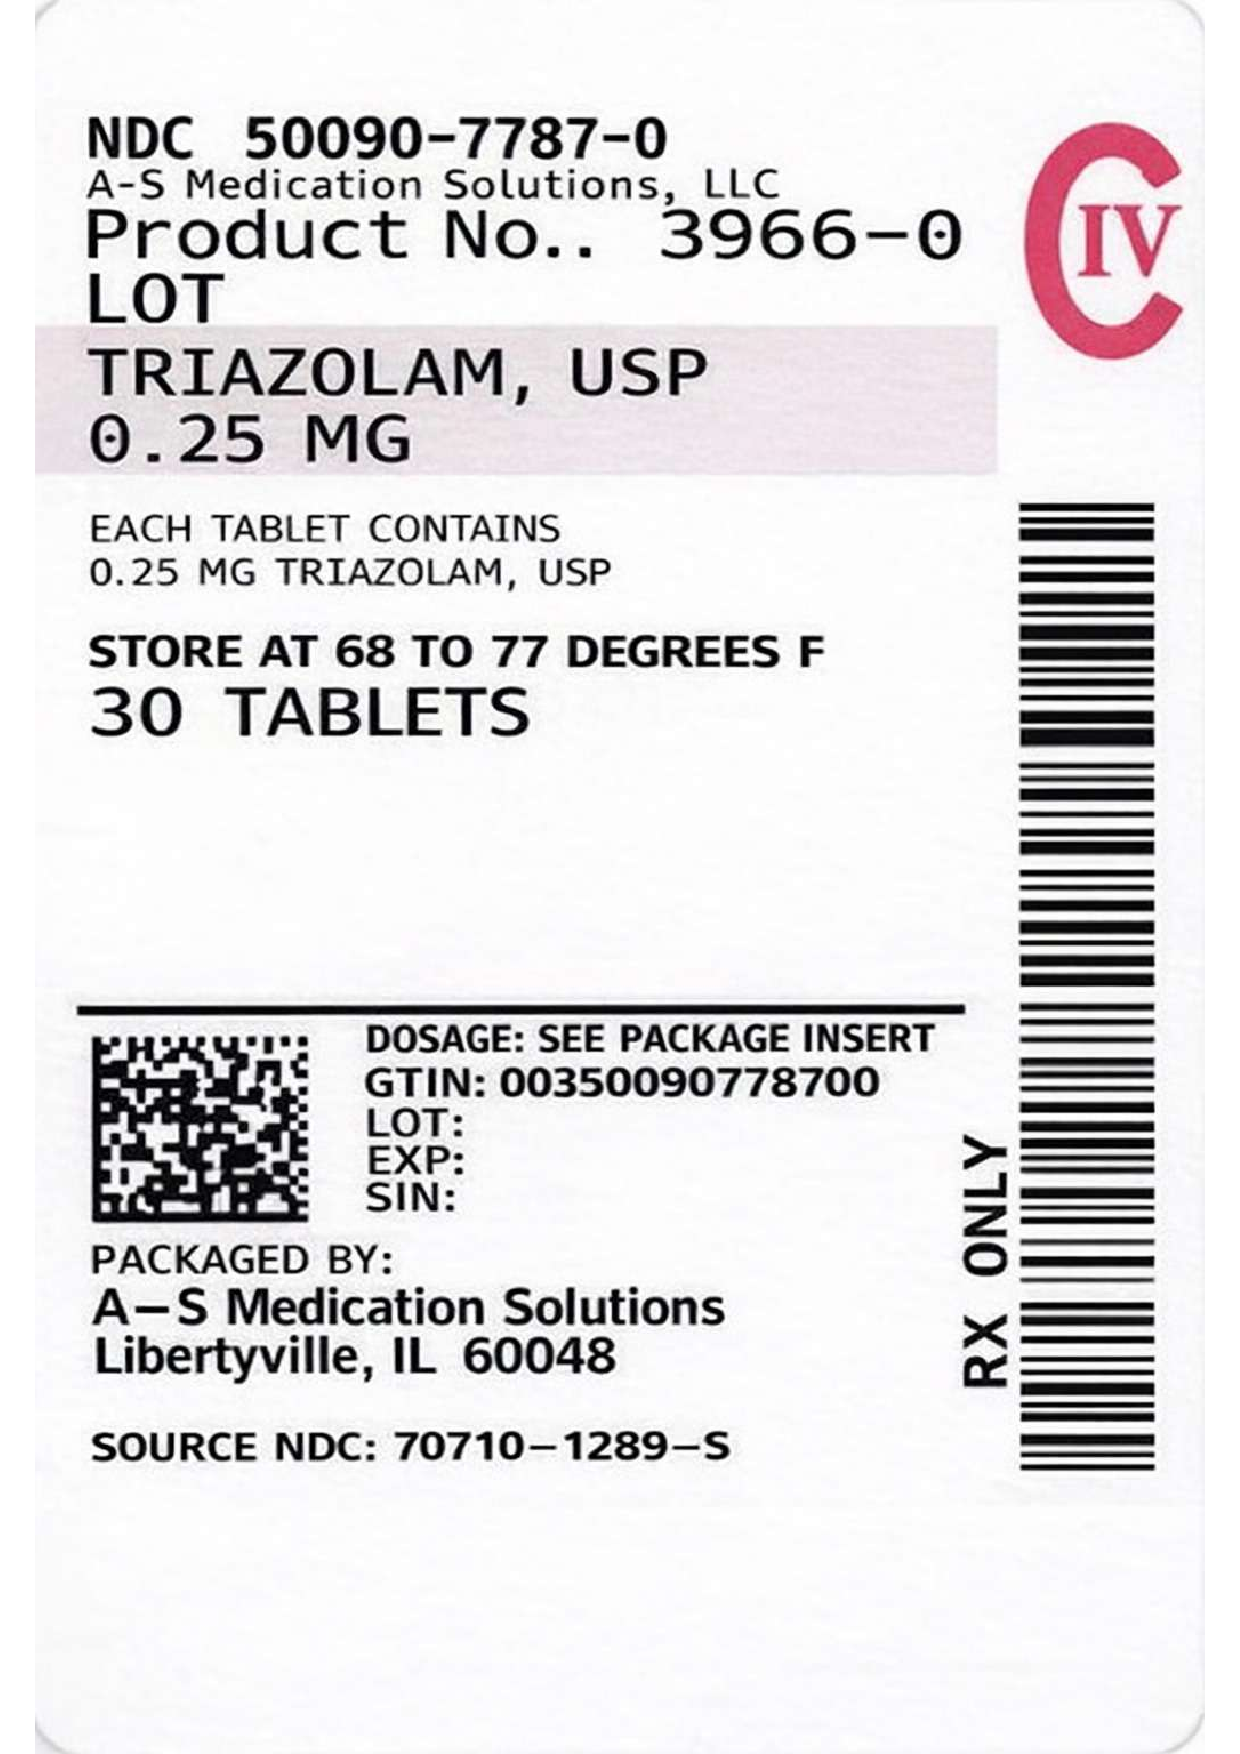
\includegraphics[width=0.4\textwidth]{Chapters/img/rotulo-exemplo.pdf}
    \caption{Exemplo de um rótulo disponibilizado pelo \emph{DailyMed} no formato SPL.}
    \label{fig:exemplo_rotulo}
\end{figure}

\begin{lstlisting}[language=XML, caption={Exemplo de informação estruturada no formato SPL.}, label={code:xml_mapping}]
<manufacturedProduct>
  <code code="50090-7787-0" codeSystem="2.16.840.1.113883.6.69"/>
  <name>Triazolam</name>
  <ingredient classCode="ACTIB">
    <quantity>
      <numerator value="0.25" unit="mg"/>
      <denominator value="1" unit="1"/>
    </quantity>
  </ingredient>
</manufacturedProduct>
\end{lstlisting}

Conforme ilustrado na Figura~\ref{fig:exemplo_rotulo}, estes documentos são disponibilizados num formato que permite a extração automática de informação. O exemplo apresentado no Código~\ref{code:xml_mapping} demonstra a presença de identificadores estruturados, como o NDC, bem como informação sobre o medicamento e respetivos ingredientes.

\paragraph{Orange Book}
O \emph{Orange Book} é a base de dados da FDA que reúne medicamentos de síntese química aprovados. No contexto do dataset, esta fonte contribui com informação regulatória e farmacêutica sobre produtos, ingredientes, formas farmacêuticas e vias de administração, podendo apoiar a identificação de relações entre medicamentos e substâncias ativas.

\paragraph{Purple Book}
O \emph{Purple Book} corresponde à base de dados de produtos biológicos licenciados pela FDA, incluindo produtos de referência, biossimilares e produtos intercambiáveis. A sua inclusão permite representar uma componente relevante do mercado farmacêutico atual, em particular terapias biológicas. Esta fonte disponibiliza informação como o \emph{BLA Number}, nomes proprietários e nomes próprios dos produtos, tipo de licenciamento e referência ao produto original.

A Tabela~\ref{tab:purple_book_sample} apresenta um pequeno excerto ilustrativo dos campos disponibilizados. Em particular, o \emph{Purple Book} disponibiliza informação sobre o tipo de licenciamento dos produtos biológicos, permitindo distinguir produtos de referência, biossimilares e produtos intercambiáveis.

\begin{table}[!ht]
\centering
\caption{Excerto de dados extraídos do \emph{Purple Book}.}
\label{tab:purple_book_sample}
\footnotesize
\begin{tabular}{l l l l l}
\hline
\textbf{\#BLA} & \textbf{Proprietary} & \textbf{Proper} & \textbf{BLA Type} & \textbf{Ref. Product} \\
\hline
125197 & Provenge & sipuleucel-T & 351(a) & N/A \\
761444 & Bilprevda & denosumab-nxxp & 351(k) Interchangeable & Xgeva \\
761449 & Tyenne & tocilizumab-aazg & 351(k) Biosimilar & Actemra \\
\hline
\end{tabular}
\end{table}

A informação proveniente destas fontes é utilizada indiretamente através dos objetos estruturados produzidos pelo \emph{MedJsonify}, que constituem a entrada do módulo de construção do grafo de conhecimento desenvolvido neste trabalho.

\subsection{Pré-processamento externo com MedJsonify}
\label{subsec:medjsonify}
Antes da construção do grafo de conhecimento desenvolvido neste trabalho, os dados provenientes das fontes regulatórias são processados pela ferramenta externa \emph{MedJsonify}~\cite{pereira2025mapping}. Esta ferramenta foi utilizada como infraestrutura pré-existente para converter ficheiros heterogéneos, como XML, TXT e CSV, em objetos JSON estruturados, bem como para aplicar métodos de reconhecimento de entidades biomédicas e \emph{entity linking}.

O papel desta ferramenta neste contexto é fornecer uma representação intermédia dos dados, na qual entidades como fármacos, ingredientes, indicações e contraindicações se encontram já parcialmente estruturadas. Estes objetos JSON constituem a entrada do módulo \emph{kg\_constructor}, responsável pelas etapas posteriores de normalização, resolução de entidades e construção dos tripletos canónicos.

\begin{figure}[H]
    \centering
    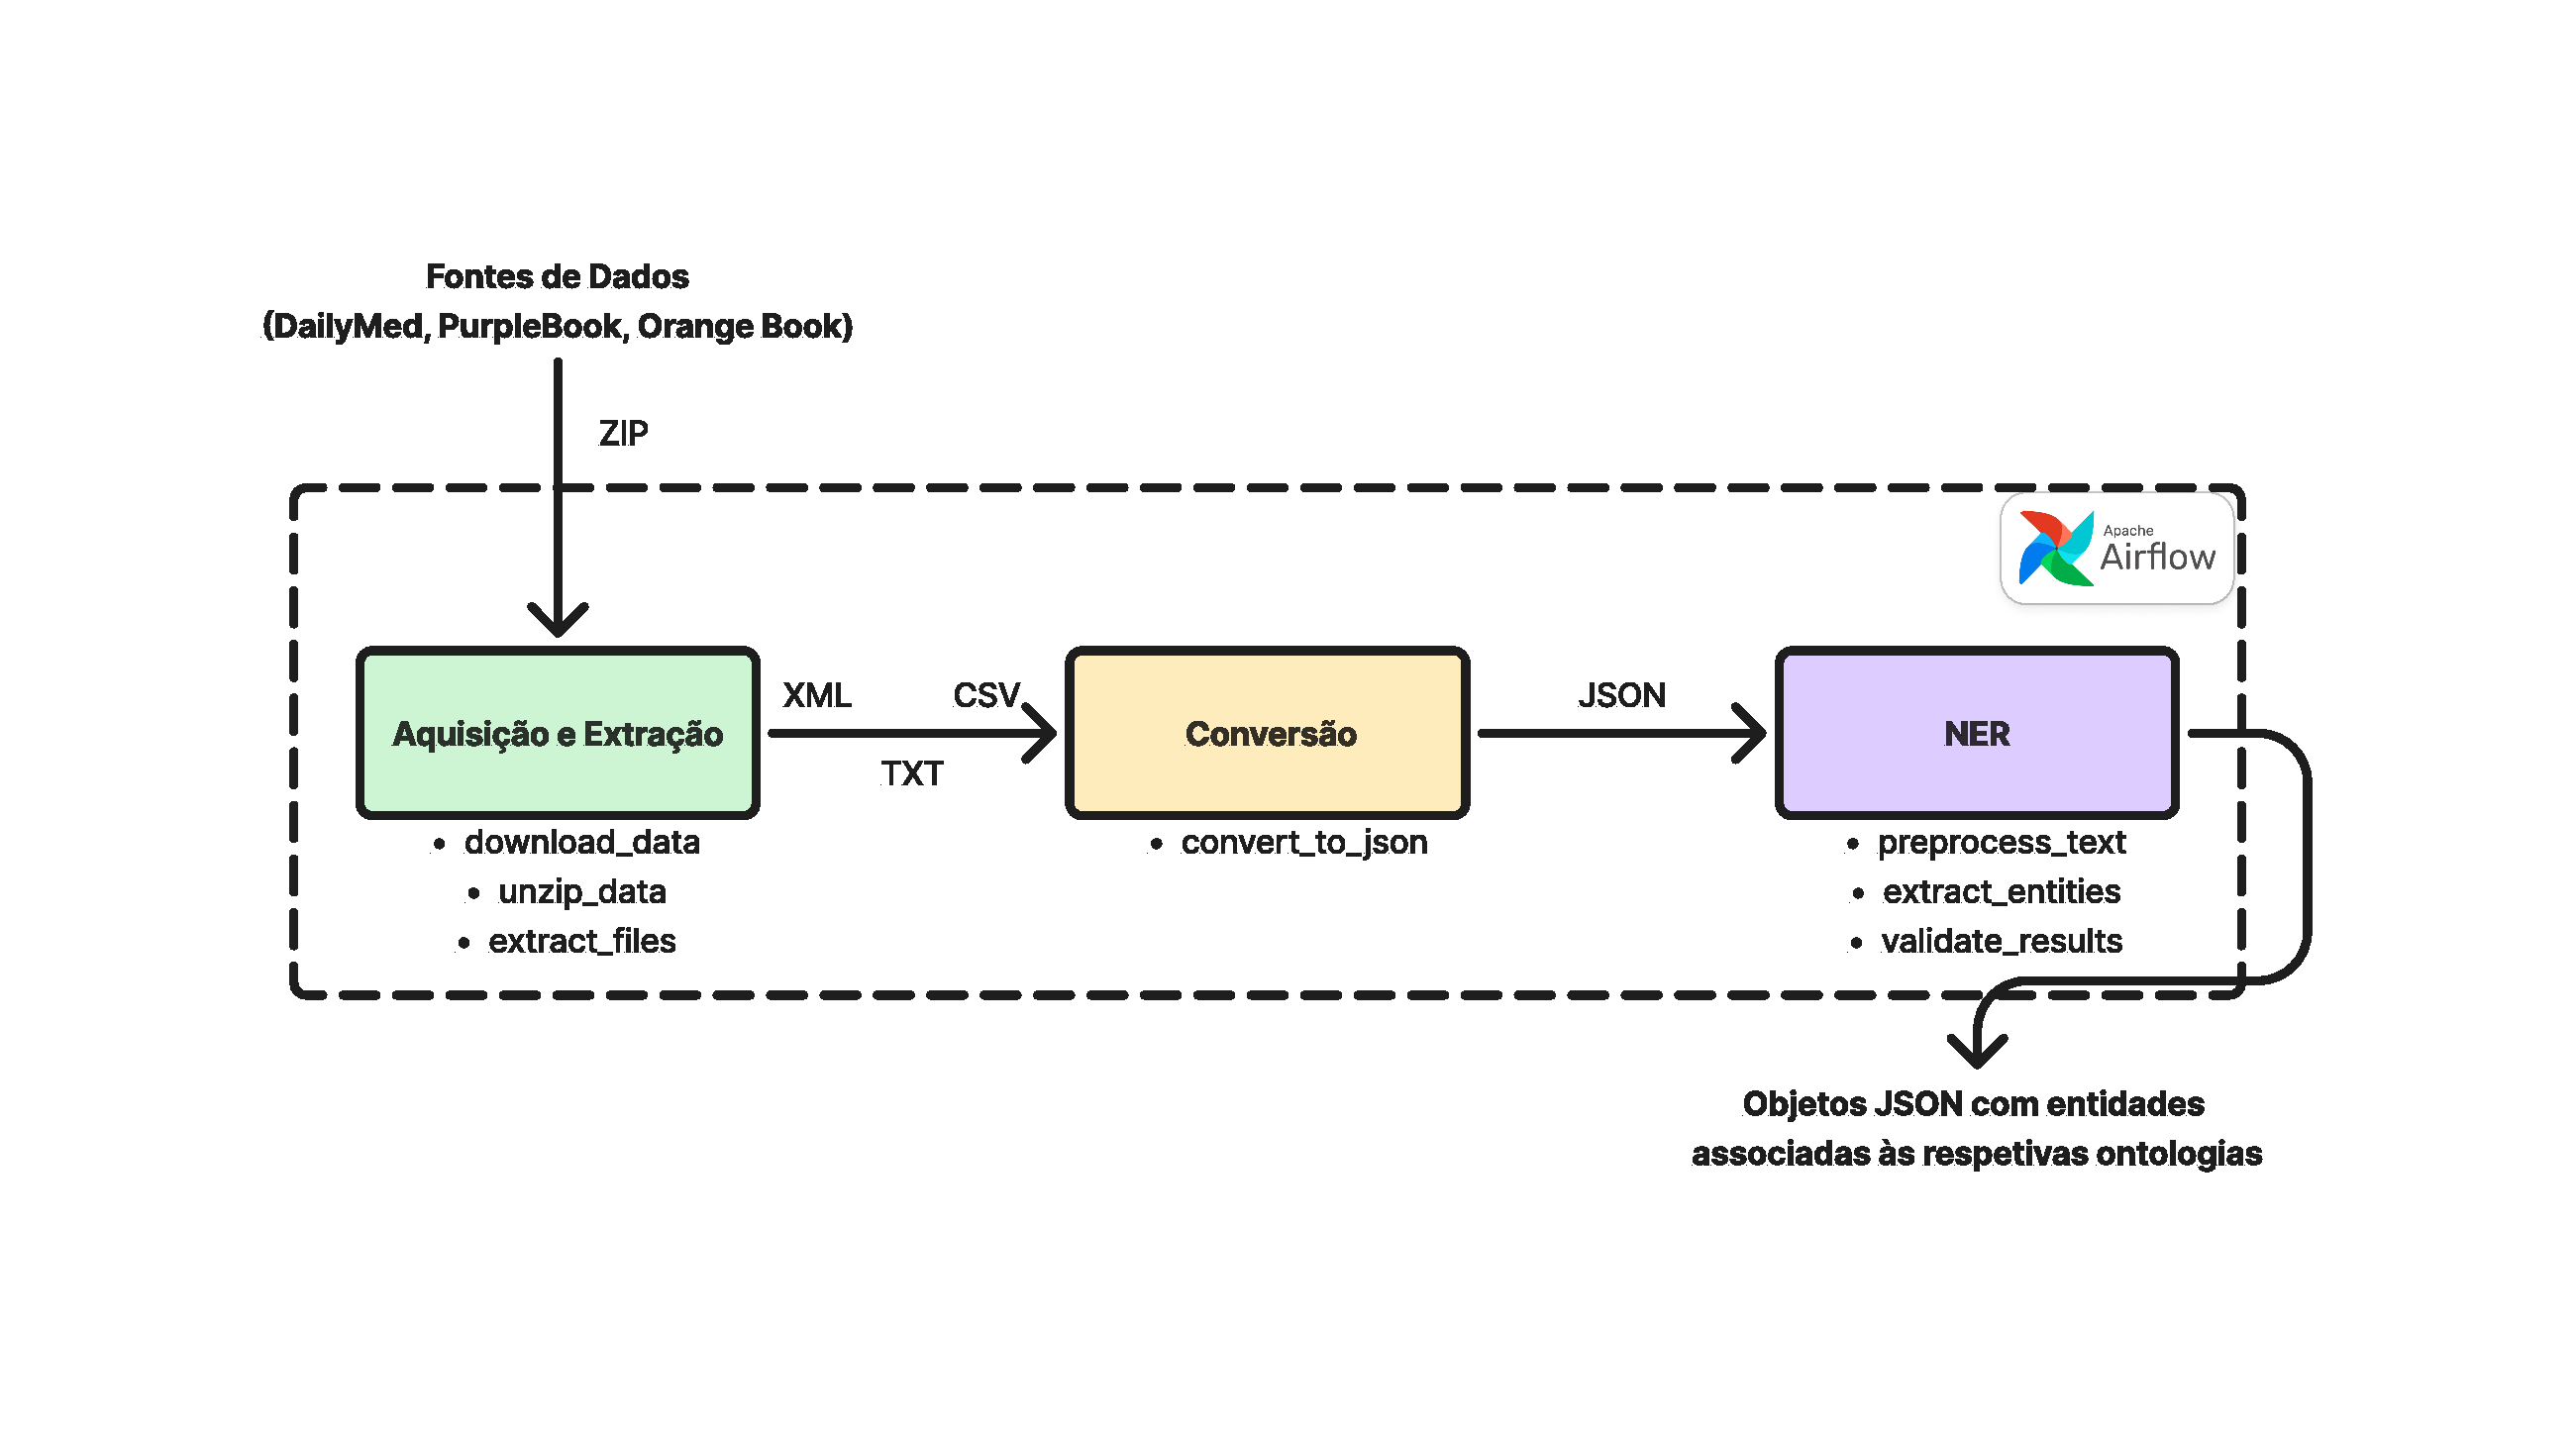
\includegraphics[
        width=\textwidth,
        trim=0cm 3cm 0cm 3cm,
        clip
    ]{Chapters/img/Pipeline.pdf}
    \caption{Visão geral do pré-processamento externo realizado pelo \emph{MedJsonify}, desde as fontes originais até à produção de objetos JSON estruturados.}
    \label{fig:pipeline_medjsonify}
\end{figure}

O Código~\ref{code:ner_outputs} apresenta exemplos simplificados dos objetos JSON utilizados como entrada. Estes outputs incluem entidades biomédicas normalizadas ou ligadas a identificadores externos, como \emph{DrugBank}, \emph{ChEBI} e \emph{Disease Ontology} (DOID), que são posteriormente convertidos em entidades canónicas no grafo de conhecimento.

\begin{lstlisting}[
language=json,
caption={Exemplo simplificado de JSON com entidades biomédicas extraídas pelo \emph{MedJsonify}.},
label={code:ner_outputs},
basicstyle=\ttfamily\small,
breaklines=true,
columns=fullflexible
]
{
  "indications": {
    "text": "Antara is indicated to reduce triglyceride levels...",
    "doid_entities": [
      {"text": "pancreatitis", "doid_id": "DOID:4989"},
      {"text": "heart disease", "doid_id": "DOID:114"}
    ]
  },
  "drug": [
    {
      "name": "Fenofibrate",
      "chebi_id": "CHEBI:5001"
    }
  ],
  "ingredients": [
    {"name": "Fenofibrate", "code": "..."}
  ]
}
\end{lstlisting}

Desta forma, o pré-processamento realizado pelo \emph{MedJsonify} estabelece a ponte entre os documentos regulatórios originais e o processo de construção do grafo desenvolvido neste trabalho. A partir desta representação intermédia, o \emph{kg\_constructor} transforma os dados em tripletos canónicos no formato \texttt{src, rel, dst}, adequados à posterior aplicação de modelos de aprendizagem relacional.

\subsection{Caracterização do Grafo de Conhecimento}
\label{subsec:caracterizacao-kg}
Após a etapa de pré-processamento externo e a aplicação dos processos de normalização e resolução de entidades, os dados são organizados sob a forma de um Grafo de Conhecimento biomédico multi-relacional. Esta representação permite estruturar diferentes tipos de entidades biomédicas, como fármacos, doenças, ingredientes e genes, bem como as relações existentes entre elas. O grafo constitui, assim, a base sobre a qual são aplicados os modelos de aprendizagem.

Ao contrário de uma representação tabular tradicional, o Grafo de Conhecimento preserva explicitamente a semântica das relações entre entidades. Esta característica é particularmente relevante no domínio biomédico, uma vez que diferentes tipos de relação representam diferentes formas de conhecimento. Uma indicação terapêutica não tem o mesmo significado que uma contraindicação, uma relação de composição farmacológica ou uma associação genética. Esta natureza justifica a utilização de arquiteturas capazes de distinguir tipos de arestas, como a \acrshort{rgcn}.

A versão final do grafo utilizada nas experiências principais corresponde ao grafo enriquecido com relações genéticas e moleculares. Esta versão combina as relações extraídas a partir dos dados regulatórios com relações provenientes de fontes biomédicas externas, permitindo introduzir uma nova camada no grafo. Assim, para além das relações entre fármacos, doenças e ingredientes, são também representadas associações entre doenças e genes.

\paragraph{Entidades (Nós)}
O grafo final inclui quatro categorias principais de entidades. Nomeadamente, fármacos, ingredientes ou substâncias ativas, doenças e genes. Os fármacos representam medicamentos ou produtos farmacêuticos identificados nas fontes de entrada, sendo normalizados preferencialmente através de identificadores externos como \emph{DrugBank}. Os ingredientes representam excipientes ou substâncias ativas associados aos fármacos, sendo identificados sempre que possível através de códigos \emph{UNII}. As patologias representam condições clínicas associadas a indicações ou contraindicações terapêuticas, sendo normalizadas através da \emph{Disease Ontology} (DOID). Por fim, os genes representam entidades obtidas a partir da integração das bases \emph{Open Targets} e \emph{DGIdb}. Estas entidades permitem representar associações doença-gene e fármaco-gene, enriquecendo o grafo de conhecimento com informação que pode ser explorada pelos modelos de recomendação.

\begin{table}[H]
\centering
\caption{Distribuição dos tipos de entidades no grafo de conhecimento final.}
\label{tab:stats_entidades}
\begin{tabular}{|l|r|}
\hline
\rowcolor[HTML]{EFEFEF}
\textbf{Tipo de entidade} & \textbf{N.º de nós} \\ \hline
Drug & 1 947 \\ \hline
Ingredient & 2 021 \\ \hline
Disease & 753 \\ \hline
Gene & 3 696 \\ \hline
\hline
\textbf{Total} & \textbf{8 417} \\ \hline
\end{tabular}
\end{table}

\paragraph{Relações (Arestas)}
As relações representam os diferentes tipos de associação existentes entre as entidades do grafo, permitindo modelar informação clínica e biomédica proveniente das diversas fontes integradas. No grafo final foram consideradas cinco categorias de relações, abrangendo associações terapêuticas, composição farmacêutica e conhecimento molecular entre doenças, genes e fármacos.

A relação \texttt{HAS\_INGREDIENT} representa a ligação entre um fármaco e os respetivos ingredientes ou substâncias ativas, modelando a composição farmacológica dos medicamentos. As relações \texttt{INDICATION} e \texttt{CONTRAINDICATION} estabelecem associações entre fármacos e doenças, distinguindo situações em que um medicamento é recomendado daquelas em que a sua utilização é desaconselhada. Para complementar a informação clínica, a relação \texttt{ASSOCIATED\_WITH\_GENE}, obtida a partir do \emph{Open Targets}, representa associações entre doenças e genes, enquanto a relação \texttt{INTERACTS\_WITH\_GENE}, integrada a partir do \emph{DGIdb}, representa interações conhecidas entre fármacos e genes. Em conjunto, estas relações permitem representar simultaneamente o conhecimento clínico e molecular no grafo de conhecimento.

\begin{table}[H]
\centering
\caption{Distribuição das relações presentes no grafo de conhecimento final.}
\label{tab:stats_relacoes}
\begin{tabular}{|l|l|r|}
\hline
\rowcolor[HTML]{EFEFEF}
\textbf{Tipo de Relação} & \textbf{src $\rightarrow$ dest} & \textbf{N.º de Arestas} \\ \hline
\texttt{HAS\_INGREDIENT} & Drug $\rightarrow$ Ingredient & 18\,349 \\ \hline
\texttt{INDICATION} & Drug $\rightarrow$ Disease & 5\,739 \\ \hline
\texttt{CONTRAINDICATION} & Drug $\rightarrow$ Disease & 2\,220 \\ \hline
\texttt{ASSOCIATED\_WITH\_GENE} & Disease $\rightarrow$ Gene & 9\,943 \\ \hline
\texttt{INTERACTS\_WITH\_GENE} & Drug $\rightarrow$ Gene & 4\,495 \\ \hline
\hline
\textbf{Total de Arestas} & & \textbf{40\,746} \\ \hline
\end{tabular}
\end{table}

A integração das relações provenientes do \emph{Open Targets} e do \emph{DGIdb} altera significativamente a estrutura do grafo de conhecimento relativamente à sua versão inicial. Para além das associações clínicas entre fármacos e doenças, o grafo passa a incorporar ligações entre doenças e genes (\texttt{ASSOCIATED\_WITH\_GENE}) e entre fármacos e genes (\texttt{INTERACTS\_WITH\_GENE}). Este enriquecimento aumenta a conectividade do grafo e introduz conhecimento adicional, permitindo representar caminhos do tipo \texttt{Drug--Gene--Disease}, potencialmente relevantes para a aprendizagem de representações mais informativas e para a recomendação de fármacos.

%%%%%%%%%%%%%%%%%%%%%% CONTINUAR AQUI %%%%%%%%%%%%%%%
\section{Preparação do Grafo para Aprendizagem}
\label{sec:preparacao-grafo-aprendizagem}
Após a construção e caracterização do Grafo de Conhecimento, é necessário transformar a sua representação numa estrutura adequada ao treino e avaliação de modelos de aprendizagem relacional. Embora o grafo seja originalmente representado através de tripletos textuais no formato \texttt{src, rel, dst}, os modelos de aprendizagem profunda operam sobre identificadores numéricos, tensores e estruturas de grafo indexadas. Por esse motivo, antes da aplicação dos modelos, é realizada uma etapa de preparação responsável por converter entidades e relações em índices, definir a tarefa experimental, criar os conjuntos de treino, validação e teste, e construir o grafo utilizado durante o treino.

Esta separação entre a construção do \acrshort{kg} e a preparação para aprendizagem é fundamental do ponto de vista metodológico. O \acrshort{kg} representa o conhecimento disponível de forma independente da tarefa, enquanto a etapa de preparação define como esse conhecimento será utilizado pelo modelo. Assim, decisões como a escolha da relação-alvo, a seleção das relações utilizadas como contexto e a divisão dos dados são realizadas apenas nesta fase, permitindo reutilizar o mesmo grafo em diferentes configurações experimentais.

Neste trabalho, a tarefa de recomendação considerada é \emph{disease-to-drug}, cujo objetivo consiste em, dada uma patologia, ordenar os fármacos candidatos de acordo com a probabilidade de estabelecerem uma associação relevante. A preparação do grafo deve, portanto, garantir que os tripletos utilizados para treino, validação e teste são definidos de forma coerente com esta tarefa, evitando \emph{leakage}, ou fuga de informação, entre os diferentes conjuntos.

\subsection{Indexação do Grafo}
\label{subsec:indexacao-grafo}
A primeira etapa da preparação do grafo consiste na sua indexação. O \acrshort{kg} produzido na etapa anterior é representado através de tripletos no formato \texttt{src, rel, dst}, nos quais as entidades e relações são identificadas por representações textuais. No entanto, para que estes dados possam ser utilizados por modelos de aprendizagem profunda, é necessário convertê-los para uma representação numérica.

Nesta etapa, cada entidade presente no grafo recebe um identificador inteiro único, permitindo construir um vocabulário de entidades. De forma análoga, cada tipo de relação é associado a um identificador numérico, formando um vocabulário de relações. Assim, um triplo textual como:
\[(\texttt{DRUGBANK:DB00945}, \texttt{INDICATION}, \texttt{DOID:2841})\]
é convertido numa representação indexada:
\[(\texttt{src\_id}, \texttt{rel\_id}, \texttt{dst\_id})\]
onde cada elemento corresponde ao identificador numérico da respetiva entidade ou relação.

A indexação mantém os identificadores textuais originais das entidades, permitindo estabelecer a correspondência entre a representação numérica utilizada pelo modelo e o grafo original. Isto facilita a validação dos dados e a interpretação das recomendações geradas.

O processo de indexação gera vários ficheiros auxiliares, apresentados na Tabela~\ref{tab:artefactos_indexacao}. Estes ficheiros são utilizados nas etapas seguintes, como a divisão dos dados, a construção do grafo de treino e a avaliação dos modelos.

\begin{table}[H]
\centering
\caption{Principais artefactos gerados durante a indexação do grafo.}
\label{tab:artefactos_indexacao}
\begin{tabular}{|l|p{9cm}|}
\hline
\rowcolor[HTML]{EFEFEF}
\textbf{Artefacto} & \textbf{Descrição} \\ \hline
\texttt{entity2id.json} & Mapeamento entre cada entidade e o respetivo identificador numérico. \\ \hline
\texttt{id2entity.json} & Mapeamento inverso, utilizado para recuperar a entidade textual a partir do identificador. \\ \hline
\texttt{rel2id.json} & Mapeamento entre cada tipo de relação e o respetivo identificador numérico. \\ \hline
\texttt{id2rel.json} & Mapeamento inverso entre identificadores numéricos e tipos de relação. \\ \hline
\texttt{entity\_types.json} & Ficheiro com o tipo inferido para cada entidade, utilizado posteriormente na definição dos conjuntos de candidatos. \\ \hline
\texttt{triples\_indexed.csv} & Versão indexada dos tripletos, contendo \texttt{src\_id}, \texttt{rel\_id}, \texttt{dst\_id} e os respetivos identificadores textuais. \\ \hline
\texttt{graph\_metadata.json} & Ficheiro com estatísticas globais do grafo, como número de entidades, relações e tripletos. \\ \hline
\end{tabular}
\end{table}


\subsection{Definição da Tarefa de Recomendação}
\label{subsec:definicao-tarefa}
A tarefa principal considerada neste trabalho é formulada como um problema de recomendação \emph{disease-to-drug}. O objetivo é, dada uma patologia, ordenar os fármacos candidatos de acordo com a probabilidade de constituírem uma associação terapêutica relevante. Esta tarefa está diretamente alinhada com o objetivo do sistema proposto, que consiste em apoiar a descoberta e o reposicionamento de fármacos através da identificação de potenciais associações terapêuticas entre doenças e fármacos.

No Grafo de Conhecimento, as indicações terapêuticas são representadas através da relação \texttt{INDICATION}, originalmente modelada no sentido \texttt{Drug} $\rightarrow$ \texttt{Disease}. Assim, um triplo da forma:
\[(\texttt{Drug}, \texttt{INDICATION}, \texttt{Disease})\]
indica que um determinado fármaco está associado a uma patologia. No entanto, durante a avaliação da tarefa de recomendação, esta relação é explorada no sentido inverso. A doença é utilizada como consulta e os fármacos constituem o conjunto de candidatos a ordenar. Desta forma, cada triplo verdadeiro \texttt{Drug --INDICATION--> Disease} é interpretado como uma associação positiva para a consulta \texttt{Disease} $\rightarrow$ \texttt{Drug}.

Formalmente, para uma doença \(d\), o modelo atribui uma pontuação a cada fármaco candidato \(m\), estimando a plausibilidade do triplo:
\[(m, \texttt{INDICATION}, d)\]

A lista de candidatos é então ordenada por ordem decrescente de pontuação, sendo esperado que fármacos verdadeiramente associados à doença surjam nas primeiras posições do ranking. Esta abordagem permite avaliar o sistema como um recomendador, uma vez que o resultado produzido para cada doença não é apenas uma classificação binária, mas sim uma lista ordenada de hipóteses.

A Tabela~\ref{tab:definicao_tarefa_recomendacao} resume os principais elementos da tarefa utilizada nas experiências.

\begin{table}[H]
\centering
\caption{Definição da tarefa principal de recomendação.}
\label{tab:definicao_tarefa_recomendacao}
\begin{tabular}{|l|p{8cm}|}
\hline
\rowcolor[HTML]{EFEFEF}
\textbf{Componente} & \textbf{Definição} \\ \hline
Tarefa & \emph{Disease-to-drug recommendation} \\ \hline
Relação-alvo & \texttt{INDICATION} \\ \hline
Sentido original do triplo & \texttt{Drug} $\rightarrow$ \texttt{Disease} \\ \hline
Consulta da recomendação & \texttt{Disease} \\ \hline
Candidatos a ordenar & \texttt{Drug} \\ \hline
Objetivo & Ordenar fármacos candidatos para uma dada patologia \\ \hline
\end{tabular}
\end{table}

Esta definição distingue a tarefa de recomendação da simples construção do grafo. O \acrshort{kg} armazena conhecimento biomédico sob a forma de tripletos, mas a tarefa experimental define como esses tripletos são utilizados para treino e avaliação. No caso deste trabalho, apenas a relação \texttt{INDICATION} é tratada como relação-alvo da tarefa de recomendação. As restantes relações do grafo são utilizadas como contexto estrutural, contribuindo para aprender melhores representações das entidades.

\subsection{Divisão dos Dados}
\label{subsec:divisao-dados}
Após a definição da tarefa de recomendação, torna-se necessário dividir os dados em conjuntos independentes de treino, validação e teste. Esta divisão é uma etapa fundamental para avaliar corretamente a capacidade de generalização do modelo, garantindo que as associações usadas para avaliação não são observadas durante o processo de aprendizagem.

Desta forma, a divisão dos dados é realizada sobre os tripletos correspondentes à relação-alvo da tarefa, isto é, sobre as associações de indicação terapêutica representadas pela relação \texttt{INDICATION}. Assim, os tripletos representados por esta relação são separados em subconjuntos de treino, validação e teste. O conjunto de treino é utilizado para ajustar os parâmetros do modelo, o conjunto de validação permite acompanhar o desempenho durante o treino e apoiar a seleção da melhor configuração, enquanto o conjunto de teste é reservado exclusivamente para a avaliação final.

Esta opção é importante, uma vez que o objetivo experimental não é reconstruir todo o grafo, mas sim avaliar a capacidade do modelo prever associações entre patologias e fármacos. Por esse motivo, apenas os tripletos da relação-alvo são divididos. As restantes relações do grafo, como \texttt{CONTRAINDICATION}, \texttt{HAS\_INGREDIENT}, \texttt{ASSOCIATED\_WITH\_GENE} ou \texttt{INTERACTS\_WITH\_GENE}, são tratadas como relações de contexto, podendo ser utilizadas para enriquecer a representação estrutural das entidades durante o treino, de acordo com a configuração experimental considerada.

A divisão segue uma proporção de 80\% para treino, 10\% para validação e 10\% para teste. A divisão dos dados é efetuada aleatoriamente, recorrendo a uma semente fixa para garantir a reprodutibilidade. Desta forma, diferentes execuções do mesmo experimento utilizam exatamente os mesmos conjuntos de treino, validação e teste, permitindo comparar de forma justa diferentes variantes do modelo.

Seja \(\mathcal{T}_{IND}\) o conjunto de tripletos de indicação terapêutica, isto é, todos os tripletos na forma \((m, \texttt{INDICATION}, d)\), onde \(m\) representa um fármaco e \(d\) representa uma doença. Este conjunto é particionado em conjuntos de treino, validação e teste:
\[\mathcal{T}_{IND}=\mathcal{T}_{train}\cup\mathcal{T}_{valid}\cup\mathcal{T}_{test}\]
com:\[\mathcal{T}_{train}\cap\mathcal{T}_{valid}=\mathcal{T}_{train}\cap\mathcal{T}_{test}=\mathcal{T}_{valid}\cap\mathcal{T}_{test}=\emptyset\]

Desta forma, cada triplo de indicação terapêutica pertence a um único subconjunto, impedindo que a mesma associação seja utilizada simultaneamente para treino e avaliação.

\subsection{Grafo Utilizado no Treino}
\label{subsec:grafo-treino}
Após a divisão dos tripletos da relação-alvo em treino, validação e teste, é necessário definir qual é a estrutura do grafo disponibilizada ao modelo durante o processo de aprendizagem. Esta distinção é necessária, uma vez que o \acrshort{kg} completo contém todas as associações conhecidas, mas o modelo não deve observar durante o treino as ligações que serão posteriormente utilizadas para validação e teste.

O grafo utilizado pelo encoder é construído a partir dos tripletos da relação-alvo pertencentes ao conjunto de treino, juntamente com um conjunto selecionado de relações de contexto. Assim, os tripletos da relação-alvo presentes nos conjuntos de validação e teste são removidos do grafo de treino, permanecendo ocultos até ao momento da avaliação. Esta estratégia permite avaliar se o modelo é capaz de atribuir pontuações elevadas a associações verdadeiras que não foram observadas durante a fase de aprendizagem.

Por relações de contexto, entendem-se as relações que não constituem diretamente o alvo da tarefa, mas que fornecem informação relevante para a aprendizagem das representações. Dependendo da configuração experimental, as restantes relações são utilizadas como informação de contexto para enriquecer a representação das entidades durante o treino. A inclusão destas relações permite que a \acrshort{rgcn} propague informação através de diferentes tipos de ligação, aprendendo embeddings que refletem não apenas as associações conhecidas, mas também a informação clínica, farmacológica e molecular representada pelas restantes relações do grafo.

Assim, o grafo utilizado no treino pode ser representado por:

\[\mathcal{G}_{train}=\mathcal{T}_{train}\cup\mathcal{C}\]

onde \(\mathcal{T}_{train}\) representa os tripletos da relação-alvo utilizados no treino e \(\mathcal{C}\) representa o conjunto de tripletos pertencentes às relações de contexto selecionadas para a experiência. Os tripletos da relação-alvo pertencentes aos conjuntos de validação e teste não são incluídos em \(\mathcal{G}_{train}\), sendo reservados apenas para a avaliação.

Além disso, nas configurações utilizadas, é possível adicionar arestas inversas ao grafo. Esta opção permite que a passagem de mensagem ocorra nos dois sentidos de cada relação, possibilitando que a informação se propague tanto da entidade de origem para a entidade de destino como no sentido inverso. Esta estratégia é particularmente relevante em grafos biomédicos, nos quais a utilidade de uma relação pode depender da capacidade do modelo explorar a vizinhança de ambas as entidades envolvidas.

\subsection{Reprodutibilidade e Validação dos Splits}
\label{subsec:reprodutibilidade-splits}
Para garantir que os resultados experimentais são comparáveis e reprodutíveis, os conjuntos de treino, validação e teste são gerados de forma determinística a partir de uma \emph{seed} fixa e guardados em ficheiros próprios. Esta estratégia permite reutilizar exatamente os mesmos splits em diferentes execuções e em diferentes modelos, evitando que variações aleatórias na divisão dos dados influenciem a comparação entre configurações experimentais.

Para além dos tripletos pertencentes a cada conjunto, é também guardada informação de metadados associados ao processo de divisão, incluindo a relação-alvo, a \emph{seed}, as proporções utilizadas e o modo de split. Esta informação permite verificar se os splits existentes são compatíveis com a configuração experimental em uso, reduzindo o risco de comparar resultados obtidos a partir de divisões diferentes dos dados.

Um aspeto central desta validação é a prevenção de fuga de informação, ou \emph{leakage}, entre os conjuntos experimentais. Na tarefa \emph{disease-to-drug}, os tripletos da relação-alvo pertencentes aos conjuntos de validação e teste não são incluídos no grafo de treino. Desta forma, o modelo não observa diretamente as associações que deverá prever durante a avaliação.

No entanto, as restantes relações do grafo podem ser utilizadas como contexto estrutural, de acordo com a configuração experimental. Esta distinção permite que o modelo explore conhecimento adicional sem aceder diretamente aos tripletos que contêm a associação do tipo \texttt{INDICATION} reservados para validação e teste.

Por fim, durante a avaliação é mantido um conjunto de positivos conhecidos, agregando as associações verdadeiras presentes nos diferentes splits. Esta estrutura será utilizada posteriormente na avaliação através de uma estratégia de \emph{filtered ranking}, evitando penalizar o modelo quando este atribui uma pontuação elevada a uma associação que também é verdadeira, ainda que não corresponda ao triplo específico em avaliação.


\section{Modelos de Recomendação}
\label{sec:modelos-recomendacao}
Após a preparação do grafo para a aprendizagem, são definidos os modelos responsáveis por atribuir pontuações a potenciais associações entre patologias e fármacos. O modelo principal é baseado numa \acrshort{rgcn}, adequada à aprendizagem em grafos multi-relacionais, uma vez que permite distinguir explicitamente os diferentes tipos de relação presentes no grafo. Esta abordagem é comparada com uma baseline \emph{content-based}, utilizada para avaliar até que ponto uma estratégia baseada em perfis de entidades consegue competir com um modelo relacional baseado em propagação de mensagens.

A comparação entre estes modelos permite analisar se a estrutura multi-relacional do grafo contribui para melhorar a qualidade das recomendações geradas.

\subsection{Modelo baseado em R-GCN}
\label{subsec:modelo-rgcn}
Neste âmbito, o modelo principal baseia-se numa \acrshort{rgcn} e é concebido especificamente para a tarefa de recomendação disease-to-drug.% A sua utilização justifica-se pela natureza multi-relacional do grafo construído, no qual diferentes tipos de arestas representam diferentes formas de conhecimento biomédico. Assim, antes de apresentar a forma como o modelo pontua associações candidatas, importa descrever como as entidades e relações são representadas e como o encoder relacional atualiza essas representações ao longo do grafo. %

\subsubsection{Representação das Entidades e Relações}
\label{subsubsec:representacao-entidades-relacoes}
O modelo principal utilizado neste âmbito é baseado numa \acrshort{rgcn}, uma arquitetura especificamente desenhada para operar sobre grafos de natureza multi-relacional. Esta escolha é adequada ao presente contexto, uma vez que as ligações entre entidades não possuem todas o mesmo significado, pelo que devem ser tratadas de forma distinta durante a aprendizagem.

Ao contrário de uma GCN convencional, que tende a tratar as arestas de forma homogénea, a \acrshort{rgcn} incorpora explicitamente o tipo de relação durante a propagação de mensagens. Assim, a atualização dos embeddings de uma entidade depende não apenas dos nós vizinhos, mas também do tipo de ligação que a conecta aos mesmos. Esta característica é particularmente relevante no domínio biomédico, uma vez que uma ligação entre um fármaco e uma patologia por indicação terapêutica tem um significado diferente de uma ligação por contraindicação ou de uma ligação entre uma patologia e um gene.

Na arquitetura utilizada, cada entidade do grafo é associada a uma representação vetorial aprendível. Durante o treino, estas representações são atualizadas através de camadas relacionais, que agregam informação proveniente das entidades vizinhas de acordo acom os tipos de relação existentes no grafo. A atualização do embedding da entidade \(i\) numa camada \(l+1\) pode ser descrita por:

\[h_i^{(l+1)}=\sigma\left(W_0^{(l)} h_i^{(l)}+\sum_{r \in \mathcal{R}}\sum_{j \in \mathcal{N}_i^r}\frac{1}{c_{i,r}}W_r^{(l)} h_j^{(l)}\right)\]

onde \(h_i^{(l)}\) representa a embedding da entidade \(i\) na camada \(l\), \(\mathcal{R}\) corresponde ao conjunto de tipos de relação, \(\mathcal{N}_i^r\) representa o conjunto de vizinhos da entidade \(i\) ligados através da relação \(r\), \(W_r^{(l)}\) é a matriz de transformação associada à relação \(r\), \(W_0^{(l)}\) corresponde à transformação da própria entidade, \(c_{i,r}\) é um fator de normalização e \(\sigma\) representa uma função de ativação.

Esta abordagem permite que o modelo aprenda transformações específicas para cada tipo de relação. Consequentemente, a informação propagada através de uma aresta \texttt{HAS\_INGREDIENT} não é tratada da mesma forma que a informação propagada através de uma aresta \texttt{ASSOCIATED\_WITH\_GENE} ou \texttt{INTERACTS\_WITH\_GENE}. Deste modo, o modelo consegue incorporar a natureza heterogénea do grafo durante a aprendizagem das representações.

Após a obtenção dos embeddings finais das entidades, é utilizado um descodificador para atribuir uma pontuação a tripletos candidatos. No contexto da tarefa \emph{disease-to-drug}, o objetivo é estimar a plausibilidade de tripletos da forma:
\[\langle m, \texttt{INDICATION}, d \rangle\]
onde \(m\) representa um fármaco candidato e \(d\) representa a doença utilizada como consulta. A pontuação atribuída pelo modelo reflete a plausibilidade de existir uma associação entre o fármaco e a patologia. Para cada patologia, todos os fármacos candidatos representados no grafo podem ser pontuados e ordenados, produzindo assim um ranking de recomendações.

Importa referir que, nesta arquitetura, o modelo não gera novos fármacos. A recomendação é realizada sobre o conjunto de fármacos já existentes no \acrshort{kg}. Assim, o foco da tarefa reside na previsão ou priorização de potenciais novas ligações entre entidades conhecidas, isto é, novas associações candidatas entre fármacos e patologias.

Durante o treino, o modelo aprende a atribuir pontuações mais elevadas a tripletos verdadeiros do que a tripletos negativos gerados artificialmente. Estes exemplos negativos são construídos através da substituição de uma das entidades do triplo por outra entidade candidata, criando associações não existentes no grafo. Desta forma, a \acrshort{rgcn} aprende a distinguir associações conhecidas de associações plausíveis mas não confirmadas, ajustando as embeddings das entidades e os parâmetros relacionais do modelo.


\subsubsection{Encoder Relacional}
\label{subsubsec:encoder-relacional}


\subsubsection{Decoder e Pontuação dos Tripletos}
\label{subsubsec:decoder-pontuacao}

\subsubsection{Treino do Modelo}
\label{subsubsec:treino-rgcn}

\subsubsection{Geração de Recomendações}
\label{subsubsec:geracao-recomendacoes-rgcn}

\subsection{Baseline Content-Based}
\label{subsec:baseline-content-based}

\section{Configurações Experimentais}
\label{subsec:configuracoes-experimentais}
Com o objetivo de avaliar o impacto dos diferentes tipos de conhecimento representados no grafo, foram definidas várias configurações experimentais. Todas as configurações mantêm a mesma tarefa principal de recomendação, isto é, a predição de ligações entre patologias e fármacos através da relação \texttt{INDICATION}. Desta forma, as diferenças observadas entre experiências podem ser analisadas em função das relações de contexto disponibilizadas ao modelo e não de alterações na tarefa de previsão.


%%%%%%%%%%%%%%%%%%%%%%%%%%%%%%%%%%%%%%%%%%%% Para o fim deste capitulo %%%%%%%%%%%%%%%%%%%%
\section{Estratégia de Avaliação e Métricas}
\label{sec:avaliacao e metrica}
Para verificar a funcionalidade do sistema, a avaliação será feita de duas formas. Através de métricas matemáticas (como o \emph{Mean Reciprocal Rank} e o \emph{Hits@k}) e através de uma análise qualitativa baseada em literatura científica para validar a veracidade clínica das hipóteses geradas.

\paragraph{Métricas de Desempenho Quantitativo}
A avaliação foca-se na tarefa de \emph{Link Prediction}, medindo a capacidade do modelo ordenar corretamente as associações verdadeiras. Para tal, serão utilizadas as métricas padrão da literatura:
\begin{itemize}
    \item \emph{Mean Reciprocal Rank} (MRR): Esta métrica avalia o \emph{rank} (posição média) da ligação na lista de recomendações geradas. Um valor de MRR próximo de 1 indica que o sistema consegue posicionar consistentemente as associações reais no topo das suas sugestões.
    
    \item \emph{Hits@k} (k=1, 3, 10): O \emph{Hits@k} quantifica a percentagem de casos em que a associação correta aparece entre os primeiros $k$ resultados sugeridos pelo modelo. O destaque atribuído ao \emph{Hits@10} justifica-se pela sua relevância para a utilidade da solução. Num cenário real de investigação, o objetivo é reduzir o espaço de pesquisa para o especialista. Ao assegurar que a resposta correta se encontra no \emph{Top-10}, garante-se que a hipótese tem uma elevada probabilidade de ser identificada e validada, minimizando o esforço de revisão manual de milhares de possibilidades.
\end{itemize}

